\documentclass[12pt,modern]{aastex61}
\usepackage{graphics,graphicx}
\usepackage{hyperref}
\usepackage{amssymb}
\usepackage{amsmath}
\usepackage{comment}
\usepackage{grffile} % checks for multiple dots in figure filenames
\usepackage{empheq} % for boxing equations
\newcommand*\widefbox[1]{\fbox{\hspace{0.2cm}#1\hspace{0.2cm}}}

%% Reintroduced the \received and \accepted commands from AASTeX v5.2
%\received{July 1, 2016}
%\revised{September 27, 2016}
%\accepted{\today}
%% Command to document which AAS Journal the manuscript was submitted to.
%% Adds "Submitted to " the arguement.
\submitjournal{AAS journals.}


\shortauthors{Bouma et al.}
\shorttitle{Binarity and Occurrence Rates}


\newcommand{\pp}{\mathcal{P}}
\newcommand{\ps}{\mathcal{S}}
\renewcommand{\a}{_{\rm a}}
\newcommand{\s}{_{\rm s}}
\newcommand{\p}{_{\rm p}}
\renewcommand{\d}{_{\rm d}}
\renewcommand{\b}{_{\rm b}}
\begin{document}
    
\title{ The effects of binarity on planet occurrence rates measured by
transit surveys}
%
\correspondingauthor{L. Bouma}
\email{luke@astro.princeton.edu}
%
\author{L. G. Bouma}
\affiliation{
    Department of Astrophysical Sciences,
    Princeton University,
    4 Ivy Lane, Princeton, NJ 08540, USA}
\author{K. Masuda}
\affiliation{
    Department of Astrophysical Sciences,
    Princeton University,
    4 Ivy Lane, Princeton, NJ 08540, USA}
\author{J. N. Winn}
\affiliation{
    Department of Astrophysical Sciences,
    Princeton University,
    4 Ivy Lane, Princeton, NJ 08540, USA}
%
%
\begin{abstract}
%

Wide-field surveys for transiting planets, such as the NASA
{\it Kepler} and {\it TESS} missions, are usually conducted without
knowing which stars are binaries. Unresolved and unrecognized binary
stars give rise to systematic errors in planet occurrence rates,
including misclassified planets and miscounts in the number of
searched stars. The individual errors can have different signs,
making it difficult to anticipate the net effect on inferred
occurrence rates. Here we use simplified models of signal-to-noise
limited transit surveys to try and clarify the situation. We derive
a formula for the apparent occurrence rate density measured by an
observer who falsely assumes all stars are single. The formula
depends on the binary fraction; the mass function of the secondary
stars; and the true occurrence of planets around primaries,
secondaries, and single stars. It also takes into account the
Malmquist bias by which binaries are over-represented in
flux-limited samples. Application of the formula to an idealized
{\it Kepler}-like survey shows that for planets larger than
$2r_\oplus$, the net systematic error is of order 10\%. For smaller
planets the errors are potentially larger: the occurrence of
Earth-sized planets could be overestimated by as much as a factor of
two. One consequence is that unrecognized binaries cannot account
for the apparent discrepancy between hot Jupiter occurrence
rates measured by transit and RV surveys. We also show that if
high-resolution imaging reveals a transit host star to be a binary,
the planet is usually more likely to orbit the primary star than the
secondary star.
%
\end{abstract}
%
\keywords{
    methods: data analysis ---
    planets and satellites: detection ---
    surveys}
%
%

%%%%%%%%%%%%%%%%%%%%%%%%%%%%%%%%%%%%%%%%%%%%%%%%%%%%%%%%%%%%%%%%%%%%%%%%%%%%%%%
%%%%%%%%%%%%%%%%%%%%%%%%%%%%%%%%%%%%%%%%%%%%%%%%%%%%%%%%%%%%%%%%%%%%%%%%%%%%%%%

\section{Introduction}

One of the goals of exoplanetary science is to establish how common,
or rare, are planets of various types.  Knowledge of planet occurrence
rates is helpful for inspiring and testing theories of planet
formation, designing the next generation of planet-finding surveys,
and simply satisfying our curiosity about other worlds.  One method
for measuring occurrence rates is to monitor the brightnesses of many
stars over a wide field, seeking evidence for planetary transits.
Measuring occurrence rates using this method was the highest priority
of the NASA {\it Kepler} mission.  Great strides have been made in the
analysis of {\it Kepler} data, including progress towards measuring
the fraction of Sun-like stars that harbor Earth-like planets~\citep{
  youdin_exoplanet_2011,petigura_prevalence_2013,dong_fast_2013,
  foreman-mackey_exoplanet_2014,burke_terrestrial_2015}

A lingering concern in occurrence rate studies is that in most cases,
investigators have assumed that all of the sources of light that were
monitored are single stars~\citep[\textit{e.g.},][]{
  howard_planet_2012,fressin_false_2013,
  dressing_occurrence_2015,burke_terrestrial_2015}. In reality many of
them are unresolved multiple-star systems, especially binaries.
Unrecognized binaries cause numerous systematic errors in the
planetary occurrence rates.  For example, when there is a transiting
planet around a star in a binary, the additive constant light from the
second star reduces the fractional loss of light due to the planet.
This ``flux dilution'' makes transit signals harder to detect and
lowers the number of detections.  On the other hand, in a binary there
two opportunities to detect transiting planets, which could increase
the overall number of detections.

At the outset of this study it was not clear to us whether the neglect
of binaries was a serious issue at all, or even whether the net effect
of all the errors is positive or negative.  The goal of this study was
to clarify the various sources of error and provide a framework for
dealing with these issues.  In this spirit, most of our models are
idealized and analytic, and we do not attempt a detailed correction of
the results from {\it Kepler} or any other real transit survey.
Our goal is to estimate the order of magnitude of the effects,
assuming the survey is signal-to-noise limited, and given the true
underlying planet occurrence rates.

This paper is organized as follows.  The next section enumerates the
various errors that arise from unrecognized binaries.  Then in
Section~\ref{sec:simplest}, we develop an idealized model of a transit
survey in which all planets have identical properties, and all stars
are identical except that some fraction are in binary systems.  This
simple model motivates the derivation of a general formula, given in
Section~\ref{sec:general_formula}, that allows for more realistic
stellar and planetary populations.  We use this formula in
Section~\ref{sec:more_complicated} to explore more complicated but
nevertheless still analytic models.  In Section~\ref{sec:discussion}
we discuss the errors due to unrecognized binaries for specific cases
of current interest: the occurrence of Earth-like planets; the
apparent discrepancy between hot Jupiter occurrence rates in different
surveys; and the shape of the ``evaporation valley'' in the planet
radius distribution that was brought to light by
\citet{fulton_california-_2017}.  We review all the results in
Section~\ref{sec:conclusion}.


\section{Understanding the errors}
\label{sec:concept}

Imagine a group of astronomers that wants to measure the mean number of
planets of a certain type per star of a certain type.  They perform a
wide-field photometric search for planets that transit, and discover
all for which
\begin{equation}
\frac{\delta_{\rm obs}}{\sigma}
  = ({\rm constant}) \cdot \delta_{\rm obs} L_{\rm sys}^{1/2} d^{-1}
> \left(\frac{{\rm S}}{{\rm N}}\right)_{\rm min}.
\label{eq:S_N_thresh}
\end{equation}
Here the signal S is the observed transit depth $\delta_{\rm obs}$, in
units of relative flux.
%LB: we don't introduce r or R because they are system-specific.
%For single stars, $\delta_{\rm obs} \approx (r/R)^2$; for binaries,
%flux dilution $\mathcal{D}$ lowers the observed depth to
%$\delta_{\rm obs} \approx \mathcal{D} (r/R)^2$. 
The noise N is the uncertainty in the determination of the flux ratio
of the star inside and outside of transits.  Throughout this paper we
will assume the photometric uncertainty to scale as the inverse square
root of the number of photons collected from the source, {\it i.e.},
the dependence on stellar properties is $\sigma \propto (L_{\rm
sys}/d^2)^{-1/2}$, where $L_{\rm sys}$ is the luminosity of the
stellar system and $d$ is its distance from Earth.
% The solid angle coverage, telescope area, and
% survey duration are in the ``constant'' term of
% Equation~\ref{eq:S_N_thresh}.  The transit duration also affects
% detectability, but we omit it in this work for brevity.

The astronomers then assume that all stars are single.  In particular
they do not have accurate enough parallaxes to tell that some of the
stars are apparently overluminous.  They want to compute the number of
planets with size $r$ per star of mass $M$.  If the total number of
stars for which such planets could be detected ($N_\star$) and the
number of detected planets ($N_{\rm det}$) are both large, then the
astronomers' estimate for the occurrence rate ($\Lambda$) is simply
\begin{equation}
\Lambda = \frac{N_{\rm det}}{N_\star}
                    \times \frac{1}{p_{\rm tra}},
\label{eq:occ_rate_simple}
\end{equation}
where $p_{\rm tra}$ is the geometric transit probability, needed to
account for the fact that most planetary orbits are not aligned close
enough with our line of sight to produce transits.

There are many potential pitfalls in this calculation.  Some genuine
transit signals are missed even if they formally exceed the
signal-to-noise threshold, because of the probabilistic nature of
transit detection.  Planets can be misclassified due to statistical
and systematic errors in the catalogued properties of the stars.  Some
apparent transit signals are spurious, arising from noise fluctuations
or failures of ``detrending'' the astrophysical or instrumental
variations in the photometric signal.  Poor angular resolution leads
to blends between eclipsing binary stars and other stars along nearly
the same line of sight, producing signals that mimic those of
transiting planets.

We will focus exclusively on the subset of problems that arise from
the fact that many stars exist in gravitationally bound binary
systems.  Even with this narrow focus, there are numerous sources of
error.  All three of the quantities in
Equation~\ref{eq:occ_rate_simple} are subject to observational bias:
\begin{enumerate}
%    
    \item The number of planets, $N_{\det}$, is actually the number of
      detected planets that {\it appear} to have size $r$, orbiting
      stars that {\it appear} to have mass $M$.  Whenever the
      planet-hosting star is part of a binary,
%    
    \begin{itemize}
        \item the planet's size will be misclassified because of the
          reduction in the amplitude of the photometric signal;
%        
        \item the host star's properties could be misclassified
          because its light is combined with a second star of a
          different spectral type.
%        
    \end{itemize}
%    
    \item The apparent number of stars that were searched, $N_\star$,
      is biased
%    
    \begin{itemize}
%        
        \item toward lower values, because it does not include all of
          the secondary stars that were searched for transiting
          planets;
%        
        \item toward higher values, because some of the stars that
          appeared to be suitably small and bright to detect the
          desired type of planet are in fact binaries for which the
          amplitude of the photometric signal would be reduced to an
          undetectable level.
%        
    \end{itemize}
%    
    \item The transit probability $p_{\rm tra}$, which scales with the
      stellar mean density as $\rho^{-1/3}$, is biased because the
      planet-hosting star could be misclassified.
%    
\end{enumerate}

Two other problems that may arise are not represented in
Equation~\ref{eq:occ_rate_simple}.  One is astrophysical: the true
occurrence rate of the desired type of planet may depend on whether
the host is a single star, the primary star of a binary, or the
secondary star of a binary.  Such differences could be caused by the
requirement for long-term dynamical stability, or differences in the
planet formation process.  When the search sample includes both
singles and binaries, the detected planets are thereby drawn from
different occurrence 
distributions~\citep[{\it e.g.},][]{
    wang_occurrence_2015,kraus_impact_2016}.

The other problem is an observational effect.  Even after the
astronomers learn about binaries and attempt to correct for their
presence, they must realize that the ratio of binaries to single stars
in the searched sample will differ from that in a volume-limited
sample due to a type of Malmquist bias.  Binaries have a higher total
luminosity than either the primary or secondary star would have on its
own.  This means that the binaries are searchable for transit signals
of a given amplitude at greater distances from the Earth.  The
binaries in a sample of apparently searchable stars are therefore
drawn from a larger search volume than the single stars.

Planet occurrence rates are often presented as two-dimensional density
functions in the space of planet radius and orbital period.
Thankfully none of the errors we have enumerated lead to errors in the
period distribution.  When more than one transit is detected (as is
usually required by the surveyors), the orbital periods can be
measured without ambiguity regardless of whether the host star is
single or one member of a binary.  Hence in what follows, we focus on
the radius distribution and assume the periods are measured without
significant uncertainty.

Given all of the confusing and opposing sources of error, we will
proceed in stages. We start from a barebones model in which everything
can be written down on the back of a napkin, and build up to an
analytic model allowing for generality in the distribution of the
binaries and the planets they host.  We consider only corrections to
the occurrence as a function of planetary radius, and not orbital
period (the other key variable in transit studies), because when
multiple transits are detected the period can be directly measured
regardless of whether the host star is single or part of a binary.


%%%%%%%%%%%%%%%%%%%%%%%%%%%%%%%%%%%%%%%%%%%%%%%%%%%%%%%%%%%%%%%%%%%%%%%%%%%%%%%
%%%%%%%%%%%%%%%%%%%%%%%%%%%%%%%%%%%%%%%%%%%%%%%%%%%%%%%%%%%%%%%%%%%%%%%%%%%%%%%

\section{Simple models}
\label{sec:simplest}

\subsection{One type of star, one type of planet}
\label{sec:model_1}

\begin{figure}[!tb]
    \begin{center}
        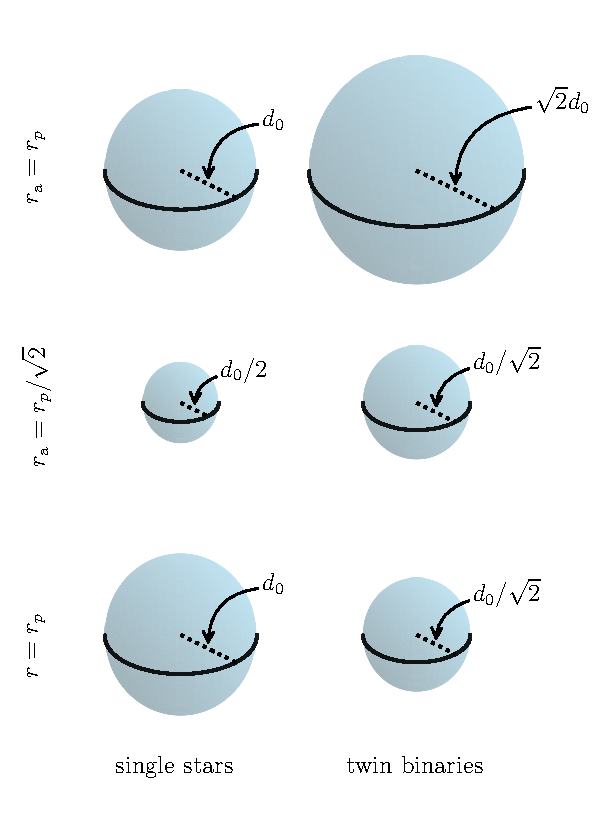
\includegraphics[width=0.6\textwidth]{figures/visualize_volumes.pdf}
    \end{center}
    \caption{
        Searchable volumes for single stars ({\it left}) and twin
        binaries ({\it right}), assuming that all stars have the same
        mass, radius, and luminosity, and that all planets have the
        same radius $r=r\p$.
        {\it Top:} At an apparent radius $r\a=r\p$, the observer
        searched twin binaries out to a distance $\sqrt{2}\times$ that
        of single stars.  Because of dilution, there are no planets in
        twin binaries with $r\a=r\p$.
        {\it Middle:} At $r\a=r\p/\sqrt{2}$, the maximum searchable
        distances are half those at $r\a=r\p$.  The only detected
        planets with $r\a=r\p/\sqrt{2}$ orbit twin binaries.
        {\it Bottom:} Planets with a true radius $r=r\p$ are
        searchable to a maximum distance $d_0$ around singles, and
        $d_0/\sqrt{2}$ around twin binaries.
    }
    \label{fig:model_1_volumes}
\end{figure}

Since the effects of binarity are most pronounced when the two
components are similar, we begin by considering a universe in which
all stars are identical, with mass $M$, radius $R$, and luminosity
$L$.  Some fraction of them exist in twin binaries. All planets have
size $r\p$.  In this scenario, stars are never misclassified because
the combined light of a binary has the same color and spectrum as a
single star.  We further assume that planets occur around single stars
and members of binaries at the same rate, $\Lambda(r\p)$.

The only type of planet in this universe produces a transit signal of
amplitude $\delta_{\rm obs} = (r\p/R)^2$ when the host is a single
star.  Our naive observers try to measure the occurrence rate of these
planets.  They identify all the ``stars'' in their sample that appear
to be searchable for such a signal, given the size of their telescope.
These transits are detected within a certain maximum 
distance~\citep[see][]{pepper_using_2003,pepper_searching_2005}, which from
Equation~\ref{eq:S_N_thresh} scales as
\begin{equation}
  d_{\rm max} \propto \delta_{\rm obs} \cdot L_{\rm sys}^{1/2}.
  \label{eq:dmax}
\end{equation}
Assuming that stars are uniformly distributed in space, the number of
searchable stars $N_\star$ is then proportional to
\begin{equation}
    N_\star \propto n_i \delta_{\rm obs}^3 L_{\rm sys}^{3/2},
\label{eq:N_searchable_prop}
\end{equation}
where $n_i$ is the number per unit volume of single stars, or
binary systems. 
 
This selection process inadvertently admits some binaries.  Since the
binaries are twice as luminous as singles, they are included out to a
distance that is larger by a factor of $\sqrt{2}$, and if they have
transiting planets then the signals have an amplitude of
$(r\p/R)^2/2$.  To detect this half-strength signal, the observers
need the noise level to be lower by a factor of two, which means the
flux must be four times higher than that of a single star at distance
$d_0$.  This is true of single stars within a distance $d_0/2$, and
binaries within a distance $d_0\sqrt{2}/2$.
Furthermore the observers will consider any such shrunken signals to
represent planets of a different type, smaller in radius by a factor
of $\sqrt{2}$. These searchable volumes are illustrated in 
Figure~\ref{fig:model_1_volumes}.

Putting it all together, the {\it apparent} occurrence rate of planets
of radius $r\p$ will be
\begin{equation}
    \Lambda\a(r\p) = 
        \frac{\Lambda(r\p)~n\s d_0^3}
        {n\s d_0^3 + n\b (d_0\sqrt{2})^3}
\end{equation}
where $n\s$ and $n\b$ are the number densities of single stars and
binary stars, respectively, in the local neighborhood.  This apparent
rate is larger than the true rate by a factor
\begin{equation}
    \frac{\Lambda\a(r\p)}{\Lambda(r\p)} = 
        \frac{1}{1 + 2^{3/2}(n\b/n\s)}.
    \label{eq:correction_rp}
\end{equation}
The observers will also claim to have discovered a new type of planet
with radius $r\p/\sqrt{2}$ and an occurrence rate given by
\begin{equation}
\label{eq:correction_diluted_rp}
    \frac{\Lambda\a(r\p/\sqrt{2})}{\Lambda(r\p)}
    =
    \frac{2n\b (d_0\sqrt{2}/2)^3}
      {n\s (d_0/2)^3 + n\b (d_0\sqrt{2}/2)^3}
    =
    \frac{2\cdot2^{3/2}(n\b/n\s)}{1 + 2^{3/2}
    (n\b/n\s)}.
\end{equation}

\begin{figure}[!tb]
    \begin{center}
        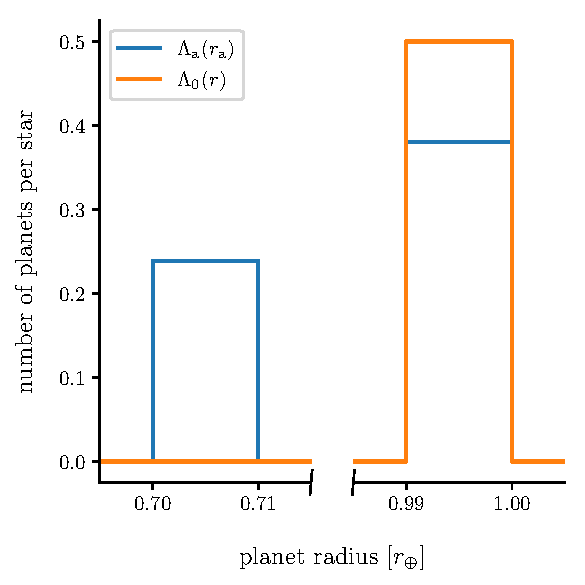
\includegraphics[width=.6\textwidth]{figures/occ_rate_vs_radius_model_1_brokenx.pdf}
    \end{center}
    \vspace{-0.5cm}
    \caption{
        Apparent occurrence rate $\Lambda\a$, and occurrence rate for
        singles $\Lambda_0$, for a model with one type of star, one
        type of planet, and twin binaries (same as
        Figure~\ref{fig:model_1_volumes}).  We assume a twin binary
        fraction of $0.05$, and that single, primary, and secondary
        stars host planets at equal rates.  If the true planet radius
        is $r\p$, all planets detected in binaries will have apparent
        radii $r\a = r\p/\sqrt{2}$; Equation~\ref{eq:ratios} gives the
        normalizations.
    }
    \label{fig:occ_rate_model_1}
\end{figure}

We can now assess the severity of these errors, given the
binary-to-single ratio $n\b/n\s$. For stars with masses from 0.7 to
1.3~$M_\odot$, \citet{raghavan_survey_2010} found the multiplicity
fraction to be 0.44, where multiplicity fraction is defined as
the fraction of systems in a volume-limited sample that are multiple.
Since we assume all multiple systems are binaries, this implies
\begin{equation}
    \frac{n\b}{n\s + n\b} \approx 0.44,
\end{equation}
which corresponds to a specific $n\b/n\s$.  Of course not all of these
binaries are close to being ``twin'' binaries as we have assumed in
our simple calculation. Perhaps only a tenth of them have pairs of
stars close enough in their basic properties to produce errors as
significant as those we have been considering.  Thus, an appropriate
estimate for $n\b/(n\s+n\b)$ is of order $0.05$, leading to
\begin{equation}
    \frac{\Lambda\a(r\p)}{\Lambda(r\p)} = 0.87,~~
    \frac{\Lambda\a(r\p/\sqrt{2})}{\Lambda(r\p)} = 0.26.
    \label{eq:ratios}
\end{equation}
All together the various effects produce biases of order 10\% in the
occurrence rates.  We will see that this level of error is
characteristic of many of our more complicated models, as well.


\subsection{Formula Based on Apparent Rate Density}
\label{sec:model_1_density}

There is a different way to conceptualize the preceding results that
will be useful in the subsequent discussion.  Here we broaden the
discussion to consider a spectrum of planet sizes, by introducing the
occurrence rate density
\begin{equation}
    \Gamma(r) \equiv \frac{d\Lambda}{dr},
\end{equation}
the average number of planets per star per unit planet radius.

To clarify our terminology, we define ``apparent properties'' as the
properties that one would infer about a system under the assumption
that the host star is single. For instance, the  ``apparent planet
radius'', $r\a$, is the planet radius that one would infer from a
transit signal, assuming that the host star is single.  The observed
transit depth is given by the ratio of the apparent planet radius and
the apparent stellar radius, $R\a$:
\begin{equation}
  \delta_{\rm obs}
  = \left(\frac{r\a}{R\a}\right)^2
  = \left[{r\over R_{\rm host}}\right]^2\times {L_{\rm host} \over
          L_{\rm sys}},
  \label{eq:delta_obs_general} 
\end{equation}
for $r$ the planet radius, $R_{\rm host}$ ($L_{\rm host}$) the host
star's radius (luminosity), and $L_{\rm sys}$ the entire system's
luminosity. This gives $r\a=r\p/\sqrt{2}$ in our ``twin binary''
model.

With this definition we may say that naive observers are measuring
$\Gamma\a(r\a)$, the apparent occurrence rate density of planets with
an apparent radius of $r\a$.  Analogous to
Equation~\ref{eq:occ_rate_simple},  
\begin{equation}
  \Gamma\a(r\a) = \frac{n_{\rm det}(r\a)}{N_\star(r\a)}
      \times \frac{1}{p_{\rm tra}},
\label{eq:apparent_rate_density}
\end{equation}
where $n_{\rm det}$ is the number of detected planets, per unit $r\a$,
with apparent radius $r\a$.  In
Equation~\ref{eq:apparent_rate_density}, we neglect the dependence on
stellar mass since all stars in this model have the same properties.
Since $\delta_{\rm obs}$ and $r\a$ are related by $R\a$, which is
simply assumed by an observer, measuring $\Gamma\a(r\a)$ is equivalent
to measuring the true occurrence rate density of {\it transit signals}
of amplitude $\delta_{\rm obs}$.

Let us evaluate the contributions to $n_{\rm det}$ from singles and
binaries.  As in the previous subsection, for each apparent planet
radius $r\a$, the observers select $N_\star(r\a)$ unresolved
point-sources on sky, based on Equation \ref{eq:dmax}.  If we let $\mu
\equiv N\star^{\rm b}(r\a)/N_\star^0(r\a)$ be the ratio of the number
of searchable binary systems to single systems, then the number of
single and binary point-sources thought to be searchable are
\begin{equation}
  \frac{N_\star(r\a)}{1+\mu}~~{\rm and}~~\frac{\mu N_\star(r\a)}{1+\mu},
\end{equation}
respectively.  Earlier we showed that due to Malmquist bias, $\mu =
2^{3/2}(n\b/n\s)$.

We further stipulate that the true occurrence rate densities for
planets around single stars, primaries, and secondaries are
$\Gamma_0(r)$, $\Gamma_1(r)$, and $\Gamma_2(r)$, respectively.  
Then single stars contribute
\begin{equation}
  n_{\rm det}^0(r\a) = 
    {N_\star(r\a) \over {1+\mu}} p_{\rm tra} \Gamma_0(r\a)
  \label{eq:n0}
\end{equation}
planet detections per unit $r\a$.  We can similarly compute the number
of planet detections from binaries.  Since $r\p=\sqrt{2}r\a$ for
planets in twin binaries, 
\begin{equation}
  n_{\rm det}^1(r\a)\mathrm{d}r\a =
      {\mu N_\star(r\a) \over {1+\mu}} p_{\rm tra}
      \Gamma_1(\sqrt{2}r\a)\mathrm{d}(\sqrt{2}r\a),
	\label{eq:n1}
\end{equation}
detections come from primaries, and
\begin{equation}
  n_{\rm det}^2(r\a)\mathrm{d}r\a =
      {\mu N_\star(r\a) \over {1+\mu}} p_{\rm tra}
      \Gamma_2(\sqrt{2}r\a)\mathrm{d}(\sqrt{2}r\a),
	\label{eq:n2}
\end{equation}
from secondaries.  Here the transit probability $p_{\rm tra}$ is the
same in all three cases because the stars are all identical. 

Using Equation~\ref{eq:apparent_rate_density}, the apparent rate
density reported when ignoring binarity is
\begin{equation}
	\label{eq:formula_twin_binary}
  \Gamma\a(r\a) =
    \frac{1}{1+\mu}\,\Gamma_0(r\a) +
    \frac{\mu}{1+\mu}\,\sqrt{2}\,\Gamma_1(\sqrt{2}r\a) +
    \frac{\mu}{1+\mu}\,\sqrt{2}\,\Gamma_2(\sqrt{2}r\a).
\end{equation}
If we further assume 
\begin{equation}
	\Gamma_i=Z \cdot \delta(r\a-r\p)
\end{equation} 
as we did in the previous ``one planet" example,
the above apparent rate density reduces to
\begin{align}
    \Gamma\a(r\a) &= Z \left[
    \frac{1}{1+\mu} \cdot
    \delta(r\a-r\p)  +
    \frac{2\mu}{1+\mu} \cdot
    \delta\left(r\a-\frac{r\p}{\sqrt{2}} \right) \right].
    \label{eq:model_1_apparent_rate_density}
\end{align}
Integrating over $r\a$, this yields
\begin{equation}
	\Lambda\a(r_{\rm p})=\frac{Z}{1+\mu},\quad
	\Lambda\a(r_{\rm p}/\sqrt{2})=\frac{2\mu Z}{1+\mu},
\end{equation}
which reproduce Equations~\ref{eq:correction_rp}
and~\ref{eq:correction_diluted_rp}.

\begin{comment}
    The ratio of the apparent to single star rate
    densities,
    \begin{equation}
        X_\Gamma(r) \equiv \left. \frac{\Gamma\a(r\a)}{\Gamma_0(r)}
          \right|_{r\a \rightarrow r},
    \end{equation}
    can then be evaluated as a ``correction factor''.  At the true and
    diluted planet radii, $X_\Gamma(r\p)=1/(1+\mu)$ and
    $X_\Gamma(r\p/\sqrt{2})=2\mu/(1+\mu)$.  This yields a correction
    $X_\Gamma$ of 0.87~(0.76) if the binary fraction is 0.05~(0.10).
    All together the various effects produce biases of order 10\% in the
    occurrence rates.  
\end{comment}

\begin{comment}
    \subsection{One type of star, two types of planets}

    A simple extension to the previous example helps distinguish between
    the apparent and underlying planet populations.  Consider now a
    universe that is the same as in Section~\ref{sec:model_1}, except that
    half of planets have radii $r\p$, while the other half have radii
    $r\p/\sqrt{2}$.  The rate densities are
    \begin{equation}
        \Gamma_i(r) = \frac{Z_i}{2} \left[
        \delta(r-r\p) + \delta\left(r-\frac{r\p}{\sqrt{2}}\right)
        \right], \quad {\rm for}\  i \in \{ 0,1,2 \},
    \end{equation}
    where $i=0$ corresponds to singles, $i=1$ to primaries, and $i=2$ to
    secondaries, and the $Z_i$'s are the number of planets per star of
    each type.

    Following an identical line of reasoning as in
    Section~\ref{sec:model_1}, the apparent rate density can be written
    \begin{align}
        \notag
        \Gamma\a(r\a) &=
        \frac{1}{2(1+\mu)} \left[
        Z_0 \cdot \delta(r\a - r\p)
        +
        \left[Z_0 + \mu (Z_1 + Z_2)
        \right] \cdot \delta\left(r\a - \frac{r\p}{\sqrt{2}}\right) 
        \right. \\
        &\quad\quad\quad\quad\quad\quad\quad\quad+
        \left.
        \mu(Z_1 + Z_2) \cdot \delta\left(r\a - \frac{r\p}{2}\right)
        \right].
        \label{eq:two_radii_twins}
    \end{align}
    Just as in Equation~\ref{eq:model_1_apparent_rate_density}, the
    $N_\star^0(r\a)$ terms cancel, leaving only the $\mu$ weights.
    However, there are now three detected planet sizes.  Also different is
    that two populations contribute at $r\a = r\p/\sqrt{2}$: the first
    population is singles with $r=r\p/\sqrt{2}$, and the second is twin
    binaries with $r=r\p$.  Both populations are detected out to the same
    maximum searchable distance.  More generally, at any given apparent
    radius, there will be contributions from both singles, primaries, and
    secondaries~---~but the relative weights between these contributions
    will depend on the underlying occurrence rates.
\end{comment}

%%%%%%%%%%%%%%%%%%%%%%%%%%%%%%%%%%%%%%%%%%%%%%%%%%%%%%%%%%%%%%%%%%%%%%%%%%%%%%%
%%%%%%%%%%%%%%%%%%%%%%%%%%%%%%%%%%%%%%%%%%%%%%%%%%%%%%%%%%%%%%%%%%%%%%%%%%%%%%%
\section{General formula for apparent occurrence rate}
\label{sec:general_formula}

To generalize the procedure of Section~\ref{sec:model_1_density} to binaries
with varying mass ratios, we consider an SNR-limited transit survey in which
stars can have arbitrary properties.  We assume that there are some functions
$L(M)$ and $R(M)$ that specify a star's luminosity and radius in terms of its
mass, and that the volume-limited binary mass ratio distribution, $f(q)$, is
independent of the primary's mass.  We also allow arbitrary true rate densities
for singles, primaries, and secondaries ($\Gamma_0, \Gamma_1, \Gamma_2$).  We
presume that the observers always know the true masses of singles and
primaries, and that they take the primary's properties to be those of an
unresolved binary.

Due to the varying mass ratios, we need the following modifications to Equation
\ref{eq:formula_twin_binary}:
\begin{enumerate}
%
  \item The number of binary systems with mass ratio $(q,
  q+\mathrm{d}q)$ in the selected sample is now
  (Equation~\ref{eq:dmax}):
  \begin{equation}
      {N_\star(r\a)\over{1+\mu}}\times {n_{\rm b}\over n_{\rm s}}
      \left[{L_{\rm sys}(M\a, q) \over L(M\a)}\right]^{3/2}
      f(q)\,\mathrm{d}q,
  \end{equation}
  where
  \begin{equation}
      \mu({\rm BF},M\a)= 
      %\frac{N_\star^{\rm b}(r\a)}{N_s^0(r\a)}=
      \int_0^1 {n_{\rm b}\over n_{\rm s}}\left[{L_{\rm sys}(M\a, q)
      \over L(M\a)}\right]^{3/2} f(q)\,\mathrm{d}q.
      \label{eq:mu_general}
  \end{equation}
  These should replace ${\mu N_\star(r\a)/(1+\mu)}$ in Equations
  \ref{eq:n0}--\ref{eq:n2}. Then the result needs to be integrated
  over $q$.

  \begin{figure}[!tb]
      \centering
      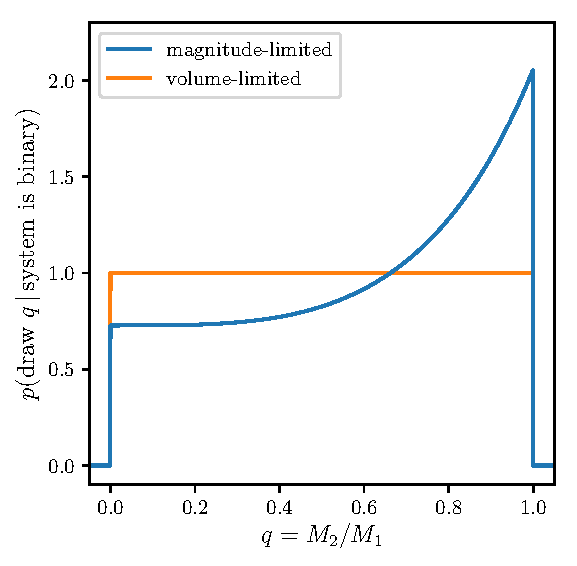
\includegraphics[width=0.6\textwidth]{figures/mass_ratio_distribution.pdf}
      \caption{
          The mass ratio distribution for a magnitude-limited sample of
          binary stars, in which the underlying volume-limited
          distribution is uniform, qualitatively similar to Figure~16 of
          \citet{raghavan_survey_2010}.  At a given observed transit
          depth, the searchable binaries in a transit survey are
          magnitude-limited. For this figure, we assume $L\propto
          M^{3.5}$
      }
      \label{fig:q_distribn_mag_limited}
  \end{figure}

  As we showed earlier, this can be understood as a Malmquist bias: in
  the magnitude-limited sample of searchable binaries, those with
  larger mass ratios are overrepresented by a factor or
  $\left[{L_{\rm sys}(M\a, q)/L(M\a)}\right]^{3/2}$ because they are
  brighter. We show this magnitude-limited mass ratio distribution
  for the flat $f(q)$ in Figure~\ref{fig:q_distribn_mag_limited}.  In
  Monte Carlo simulations of transit surveys, it is important to
  draw binaries from an appropriately biased mass-ratio
  distribution~\citep[\textit{e.g.},][]{
    bakos_hatsouth:_2013,sullivan_transiting_2015,
    gunther_new_2017}.
%
  \item The relationship between $r\a$ and $r$ are different.  From
    Equation~\ref{eq:delta_obs_general}, $r=\mathcal{D}_{1/2}r\a$ for
    primaries and secondaries, where
  \begin{equation}
      \mathcal{D}_1(q, M\a)
      = \sqrt{L_{\rm sys}(M\a, q) \over L(M\a) }
      = (1+q^\alpha)^{1/2},
  \end{equation}
  and
  \begin{equation}
    \mathcal{D}_2(q, M\a)
    = {R(qM\a)\over R(M\a)}\sqrt{L_{\rm sys}(M\a, q) \over L(qM\a)} 
    = q (1+q^{-\alpha})^{1/2}.
  \end{equation}
  So $\sqrt{2}r\a$ in Equations~\ref{eq:n1} and~\ref{eq:n2} needs to be
  replaced with $\mathcal{D}_1r\a$ and $\mathcal{D}_2r\a$, respectively.

  \item The transit probability around secondaries are smaller than
  that around primaries, the latter of which is the same as
  primaries under our assumption. At a fixed orbital period, this
  changes $p_{\rm tra}$ in Equation~\ref{eq:n2} by a factor of
  \begin{equation}
    {R(qM\a) \over R(M\a)}q^{-1/3}.
  \end{equation}

\end{enumerate}

Taking these modifications into account, a general formula for the
apparent rate density follows:
\begin{align}
    \notag
    \Gamma\a(r\a,M\a) &= {1\over 1+\mu(\mathrm{BF}, M\a)}\times
    \left\{ \Gamma_0(r\a, M\a)+ 
    \frac{n\b}{n\s}
    \left[ \int_0^1 \mathrm{d}q \,
           \mathcal{D}_1^3 f(q)\cdot
          \mathcal{D}_1 \Gamma_1\left(\mathcal{D}_1r\a,
    M\a\right)\,
    \right.   
    \right. \\
    & \quad\quad\quad\quad\quad \left.\left.
    +\int_0^1 {\rm d}q\, 
         \mathcal{D}_1^3 f(q)\cdot \mathcal{D}_2 q
        \Gamma_2\left(\mathcal{D}_2r\a, qM\a\right)\cdot
    {R(qM\a) \over R(M\a)}
    q^{-1/3} \right] \right\}.
    \label{eq:general_Gamma_a}
\end{align}
We also give a more formal derivation in the
\hyperref[sec:appendix]{Appendix}.
With the definition of $\mu$ in Equation~\ref{eq:mu_general},
Equation~\ref{eq:general_Gamma_a} can also be expressed as
\begin{align}
    \notag
    \notag
    \Gamma\a(r\a,M\a)
    &= 
    {1\over 1+\mu(\mathrm{BF}, M\a)} \cdot
    \left[
       \Gamma_0(r\a, M\a)\phantom{\tilde \Gamma}\right.&\\
       &\left.+\mu(\mathrm{BF}, M\a)\cdot
       \left\langle
       \mathcal{D}_1\cdot\Gamma_1\left(\mathcal{D}_1r\a, M\a\right)
       +
       {q \mathcal{D}_2}\cdot\Gamma_2\left(\mathcal{D}_2r\a,
       qM\a\right) \cdot {R(qM\a) \over R(M\a)}q^{-1/3}
       \right\rangle
    \right],
\end{align}
where the angle brackets denote averaging over $\mathcal{D}_1^3f(q)$.
This form shows that the fraction $\mu$ and mass ratio distribution
$\mathcal{D}_1^3f(q)$ of binaries {\it in the searchable volume} are
enough to describe the contributions from binaries to $\Gamma\a$.  The
fraction $\mu$ gives the relative contributions from singles and
binaries, and $\mathcal{D}_1^3 f(q)$ weights the contributions from
binaries with various mass ratios.  The apparent rate density at each
mass ratio ({\it i.e.}, the terms in the angle brackets) is the rate
density of systems that give the apparent $(r\a, M\a)$, corrected for
the overestimated transit probability around secondaries.

%%%%%%%%%%%%%%%%%%%%%%%%%%%%%%%%%%%%%%%%%%%%%%%%%%%%%%%%%%%%%%%%%%%%%%%%%%%%%%%
%%%%%%%%%%%%%%%%%%%%%%%%%%%%%%%%%%%%%%%%%%%%%%%%%%%%%%%%%%%%%%%%%%%%%%%%%%%%%%%

\section{Realistic Star and Planet Distributions}
\label{sec:more_complicated}

We will now apply our general equation for the apparent rate density
(Equation~\ref{eq:general_Gamma_a}) to study binarity's effects in
regimes of observational interest.  In the following, we write the
rate density for each type of star, $\Gamma_i(r)$, as the product of a
shape function and a constant:
\begin{equation}
    \Gamma_i(r) = Z_i f_i(r), \quad {\rm for\ }i\in\{0,1,2\},
\end{equation}
where $i=0$ corresponds to single stars, $i=1$ to primaries of
binaries, and $i=2$ to secondaries of binaries.  The shape function is
normalized to unity.  The $Z_i$'s are each system type's occurrence
rate $\Lambda_i$, integrated over all planetary radii. In other words,
they are number of planets per single, primary, or secondary star.  We
want to consider the effects of varying not only $f_i(r)$ but also the
relative values of the $Z_i$'s.

%%%%%%%%%%%%%%%%%%%%%%%%%%%%%%%%%%%%%%%%%%%%%%%%%%%%%%%%%%%%%%%%%%%%%%%%%%%%%%%
\subsection{Power law planet radius distributions}
\label{sec:model_2}

\subsubsection{Twin binaries}
We begin introducing realism by keeping all binaries as twins, but
letting the planet radius distributions vary.  First, we assume a
power law planet radius distribution,
\begin{equation}
    \Gamma_i(r) = Z_i f(r) = Z_i r^\delta/\mathcal{N}_r,
\end{equation}
for $f(r)$ the radius shape function, and $\mathcal{N}_r$ the shape
function's normalization.  The resulting apparent rate density is 
\begin{equation}
    \Gamma\a(r\a) = \frac{r\a^\delta}{\mathcal{N}_r} \left[
    \frac{Z_0}{1+\mu}
    +
    2^{\frac{\delta+1}{2} } \frac{\mu}{1+\mu} \left(Z_1 + Z_2
    \right)
    \right],
    \label{eq:model5_apparent_rate_density}
\end{equation}
which is quite similar to the twin binary, fixed-planet case
(Equation~\ref{eq:model_1_apparent_rate_density}), except for in the
radius dependence and normalization.  As in Section~\ref{sec:model_1},
$\mu = 2^{3/2} n\b/n\s$.  If the $Z_i$'s are equal, the ``correction
factor'' relative to the rate density for singles becomes quite
simple:
\begin{align}
    \left. \frac{\Gamma\a(r\a)}{\Gamma_0(r)} 
    \right|_{r\a\rightarrow r}
    &=
    \frac{1 + 2^{\frac{\delta+3}{2}}\mu}{1 + \mu}.
    \label{eq:power_law_correction}
\end{align}
If the binary fraction is $0.1$, $\mu\approx 0.15$. Taking
$\delta=-2.92$ from \citet{howard_planet_2012},  we find
$\Gamma\a/\Gamma_0 = 1.004$.  In other words, the apparent rate
density is an {\it over}estimate compared to the rate density of
single stars, with a relative difference $\delta \Gamma_0 =
|\Gamma_0~-~\Gamma\a|/\Gamma_0$ of 0.4\%.  This is quite a small
effect!  Clearly though, it cannot apply at small radii, since $f(r)
\propto r^\delta$ diverges; \citet{howard_planet_2012}'s results
indicate that the power law planet radius distribution holds for
$r\a\gtrsim 2r_\oplus$.  It is similarly nonsensical for $f(r)$ to be
finite above some upper radius limit $r_{\rm u}$, perhaps around
$\approx 24r_\oplus$, based on the most inflated hot Jupiters.
Imposing an upper cut-off of $r_{\rm u}$ would lead to smaller values
of $\Gamma(r\a)$ down to $r_{\rm u}/\sqrt{2}$, compared to an
intrinsic power law without the cut-off.  We are not particularly
interested in this effect because there are better models for hot
Jupiter occurrence rates that we will discuss in
Section~\ref{sec:further_models}.  If the assumptions behind this
model are at all applicable to real transit surveys,
Equation~\ref{eq:power_law_correction} suggests that for $2r_\oplus
\lesssim r\a \lesssim 17r_\oplus$, binarity's impact on apparent
occurrence rates is quite small.



%%%%%%%%%%%%%%%%%%%%%%%%%%%%%%%%%%%%%%%%%%%%%%%%%%%%%%%%%%%%%%%%%%%%%%%%%%%%%%%
\subsubsection{Binaries with power law mass ratio distribution}
\label{sub:powerlaw_varying_binaries}

To check whether non-twin binaries change the preceding result, we now
assume $f(q) = q^\beta/\mathcal{N}_q$, for $\mathcal{N}_q$ the
normalization.  This changes $\mu$ (Equation~\ref{eq:mu_general}
simplifies to Equation~\ref{eq:mu_power_laws}).  It may also affect
the rate density, which could be a function of the varying stellar
mass.  Absorbing this dependence into a power law as well,
\begin{equation}
    \Gamma_i(r,M) = Z_i \times \frac{r^\delta}{\mathcal{N}_r} \times
    \frac{M^\gamma}{\mathcal{N}_M},
\end{equation}
where $Z_i$ is dimensionless, and the normalization constants carry
the units (each side has units $[r^{-1} M^{-1}]$).  We assume that
stars are a one-parameter family, given by $R \propto M \propto
L^{\frac{1}{\alpha}}$, so that a given value of $q$ determines
everything about a secondary.

We are mostly interested in the apparent rate density's radius
dependence.  Marginalizing Equation~\ref{eq:general_Gamma_a} over
apparent stellar mass, we find that when $Z_0=Z_1=Z_2$,
\begin{align}
    X_\Gamma &\equiv \left. \frac{\Gamma\a(r\a)}{\Gamma_0(r)} 
    \right|_{r\a\rightarrow r} \\
    &=
    \notag
    \frac{1}{1+\mu}
    \left[1 + \frac{1}{\mathcal{N}_q} \frac{n\b}{n\s}\times 
    \left(
    \int_0^1 {\rm d}q\,q^\beta (1+q^\alpha)^{\frac{\delta+4}{2}} +
    \right.
    \right. \\
    %isn't latex great?
    &\quad\quad\quad\quad\quad\quad\quad\quad\quad\quad
    \left.\left.
    \int_0^1 {\rm d}q\,q^{\beta+\delta+\frac{5}{3}} 
    (1+q^\alpha)^{\frac{3}{2}}
    (1+q^{-\alpha})^{\frac{\delta+1}{2}}
    \right)\right],
    \label{eq:powerlaw_vary_binary}
\end{align}
where $\gamma$ does not appear because of the marginalization over
$M\a$.  For $\alpha = 3.5$, $\beta=0$, $\gamma=0$, $\delta=-2.92$, the
summed integrals in Equation~\ref{eq:powerlaw_vary_binary} give
$(\ldots)\approx 1.50249$. %171211_model_integrals.nb
For $n\b / (n\b + n\s)=0.44$, this yields $\Gamma\a/\Gamma_0 = 1.048$;
the relative difference between the apparent rate density and the rate
density around singles is 4.8\%.  This indicates that considering only
twin binaries gave us correct intuition: for a power law radius
distribution ($2r_\oplus \lesssim r\a \lesssim 17r_\oplus$) in which
there are the same number of planets orbiting singles, primaries, and
secondaries, binarity influences apparent planet occurrence rates
around Sun-like stars at the $\sim$few percent level.



%%%%%%%%%%%%%%%%%%%%%%%%%%%%%%%%%%%%%%%%%%%%%%%%%%%%%%%%%%%%%%%%%%%%%%%%%%%%%%%
\subsection{Varying stars; broken power law planet radius distribution}
\label{sec:model_3}

\begin{figure}[!t]
    \centering
    \epsscale{1.15}
    \plottwo{figures/int_rate_density_vs_radius_model_3_rpu_22.5_manyZs.pdf}{figures/int_occ_rate_vs_radius_model_3_rpu_22.5_manyZs.pdf}
    \caption{
        {\it Left:} apparent rate density ($\Gamma\a$) and single star
        rate density ($\Gamma_0$). {\it Right:} apparent occurrence
        rate ($\Lambda\a$) and single star occurrence rate
        ($\Lambda_0$), over $0.5r_\oplus$ bins.  The true planet
        radius distribution is specified by
        Equation~\ref{eq:model3_radius_distribution}.  This model
        assumes that the observer knows the true properties of all the
        singles and primaries, and that the volume-limited mass ratios
        of secondaries are drawn from a uniform distribution. Further,
        we take $Z_0=Z_1=0.5$ throughout; $Z_0,Z_1,Z_2$ are the number
        of planets per single, primary, and secondary star.  The rate
        and rate density are related by $\Lambda|_a^b =
        \int_{a}^{b}\Gamma\,{\rm d}r$.
    }
    \label{fig:occ_rate_model_3_log}
\end{figure}

Though the details of the planet radius distribution $\Gamma_i(r)$ at
$r<2r_\oplus$ are currently an active topic of research, we can
consider how binarity affects this regime under different plausible
assumptions.  For instance, assume that the true radius shape function
is
\begin{align}
    f(r)
    &\propto
    \left.
    \begin{cases}
        r^\delta & \text{for } r\geq 2r_\oplus \\
        {\rm constant} & \text{for } r\leq2r_\oplus.
    \end{cases}
    \right.
    \label{eq:model3_radius_distribution}
\end{align}
As in the previous model, we presume that the observers know the true
properties of all singles and primaries. The masses, radii, and
luminosities of stars vary as $R \propto M \propto
L^{\frac{1}{\alpha}}$.  Our ``nominal model'' remains the same:
$\alpha=3.5$, $\beta=\gamma=0$, $\delta=-2.92$.

At apparent radii $r\a > 2r_\oplus$, the results of this model are the
same as those from Section~\ref{sub:powerlaw_varying_binaries}.  For
$r\a < 2r_\oplus$, the equations are tedious, but still tractable.
For simplicity, we insert Equation~\ref{eq:model3_radius_distribution}
into Equation~\ref{eq:general_Gamma_a}, and integrate using a computer
program. We refer the interested reader to our online
implementation\footnote{\url{https://github.com/lgbouma/binary_biases}}.
The output is validated against analytic predictions in the $r\a >
2r_\oplus$ and the $r\a < 2r_\oplus/\sqrt{2}$ regimes, and is plotted
in Figure~\ref{fig:occ_rate_model_3_log}.


\paragraph{The rate of Earth analogs} The immediately arresting result
there is a ``bump'' in the apparent rate density at $r\a < 2r_\oplus$:
the true rate for singles is less than the inferred rate.  For the
case in which secondaries host as many (half as many) planets as
single stars, this means an overestimate of the absolute occurrence
rate by $\approx 50\%$ ($\approx 25\%$).  The ``bump'' exists even for
the $Z_2/Z_0=0$ case as a $\approx 10\%$ effect.  The magnitude of
this evidently error depends strongly on the prevalence of planets
around secondaries.

\paragraph{Hot Jupiter occurrence rates} Taking
Figure~\ref{fig:occ_rate_model_3_log} and integrating the rate
density, we can compare the apparent hot Jupiter occurrence rate with
the true rate for singles.  In the most extreme case of $Z_2/Z_0=0$,
we find that $\Lambda_{{\rm HJ},0}/\Lambda_{\rm HJ,a} = 1.13$, where
\begin{equation}
    \Lambda_{\rm HJ,a} =
      \int_{8r_\oplus}^{\infty} \Gamma\a(r)\,{\rm d}r,
\end{equation}
and similarly for $\Lambda_{\rm HJ,0}$.
%occ_rate_vs_radius_model_3_withtext_Zsub2_0.00_rpu_22.5.pdf
If $Z_2/Z_0>0$, binarity affects the apparent hot Jupiter rate less:
when $Z_2/Z_0=0.5$, we find $\Lambda_{{\rm HJ},0}/\Lambda_{\rm HJ,a} =
1.06$.  We discuss this issue further in
Section~\ref{sec:further_models}.

\paragraph{Fraction of detected planets from a given source}

\begin{figure}[!t]
    \centering
    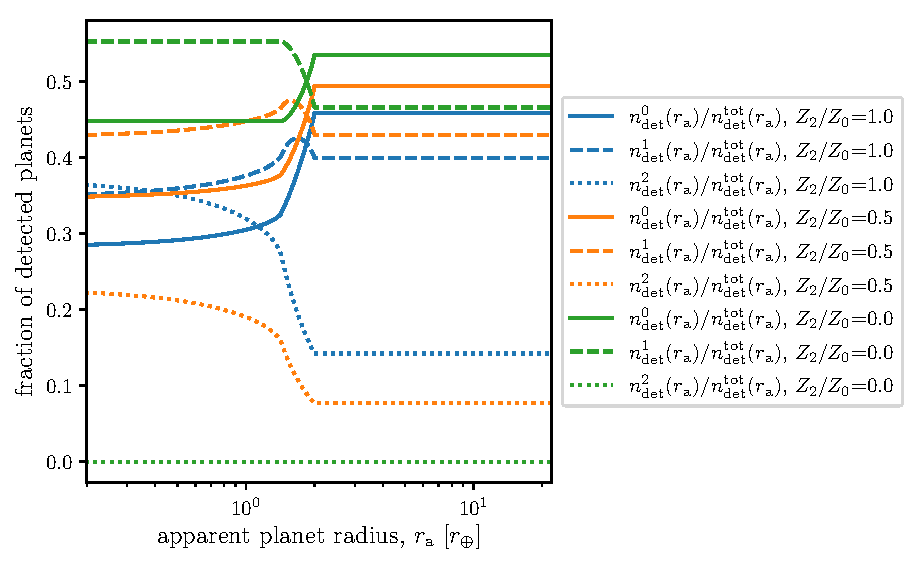
\includegraphics[width=\textwidth]{figures/ndet_vs_radius_logx_model_3_fraclines_rpu_22.5_manyZs.pdf}
    \caption{
        Fraction of detected planets at a given apparent planet radius
        coming from singles (solid lines), primaries (dashed lines),
        and secondaries (dotted lines).  Three different values for
        $Z_2/Z_0$ are selected: $1$ (blue), $0.5$ (orange), $0$
        (green).  The assumed true planet radius distribution is a
        broken power law
        (Equation~\ref{eq:model3_radius_distribution}; same as
        Figure~\ref{fig:occ_rate_model_3_log}).
    }
    \label{fig:frac_model_3}
\end{figure}

It would be nice to improve our intuition for how much the secondaries
matter.  We have the understanding that for a given true planet
radius, secondaries have a much smaller searchable volume than
primaries or singles.  Does this necessarily imply that if we are
given a detected planet with some apparent radius $r\a$, which is then
observed by high-resolution imaging to exist in a binary, that the
planet probably orbits the primary?

We explore this quantitatively in Figure~\ref{fig:frac_model_3}.  The
lines in this figure are computed using expressions given in the
appendix for the number of detections coming from singles, primaries,
and secondaries (Eqs.~\ref{eq:n_det_0},~\ref{eq:n_det_1},
and~\ref{eq:n_det_2}).

In short, the detected planet usually is more likely to orbit the
primary, but this statement depends on the number of planets orbiting
secondaries, and also on the apparent radius of the detected planet.
In the scenario that high-resolution imaging finds a system with $r\a
> 2r_\oplus$ in a binary, roughly $\sim\! 2.5\times$ more detected
planets orbit primaries than secondaries, for the $Z_2/Z_0=1$ case.
For the $Z_2/Z_0=0.5$ case, $\sim\! 5\times$ more detected planets
orbit primaries than secondaries.  So detected planets in binaries
with large apparent radii (relative to the cutoff in the intrinsic
rate density) are more likely to orbit the primary.

The situation for $r\a < 2r_\oplus$ is more nuanced.  For the $Z_2=0$
and $Z_2/Z_0=0.5$ cases, detected planets in binaries are still always
more likely to orbit the primary.  However, if there are as many
planets orbiting the secondaries as the primaries, then there is a
turn-over radius, $\approx 0.4r_\oplus$, beyond which more of the
detected planets in binaries come from secondaries: they have all been
``diluted down'' from larger true planetary radii!  Although this
(apparent) radius is at the limit of current detection sensitivities,
this effect will be interesting for future instruments to investigate.

Further, Figure~\ref{fig:frac_model_3} shows that going from apparent
radii of $2r_\oplus$ to $\approx 1.4r_\oplus$, the fraction of
detected planets with binary companions increases by $\approx 6-12\%$,
depending on the assumed value of $Z_2/Z_0$. %~\footnote{
%The increase can be derived analytically.  Let the fraction of total
%detected planets from primaries at a given apparent radius be
%$F_1(r\a)$, so $F_1(r\a) \equiv n_{\rm det}^1(r\a)/n_{\rm det}^{\rm
%tot}$.  Let the analogous quantity for secondaries be $F_2(r\a)$.  In
%the planet-less secondaries case ($F_2(r\a)=0$), one can analyze
%Eqs~\ref{eq:n_det_0} and~\ref{eq:n_det_1} semi-analytically and show
%that $F_1(2r_\oplus/\sqrt{2})/F_1(2r_\oplus) \approx 1.19$.
%check_companion_fractions.py, and LB's notes 2017/12/21.0 }.
Intuitively speaking, this ``shift'' is a feature of any radius
distribution that declines at large radii, and flattens below some
cutoff $r_{\rm c}$.  This is because (for dilution about primaries) at
apparent radii $r\a < r_{\rm c}/\sqrt{2}$, relatively more planets
will be ``diluted'' into the given $r\a$, since there are more planets
in the undiluted distribution from $r\a$ to $\sqrt{2}r\a$.  We compare
this prediction with recent observations in
Section~\ref{sec:discussion}.



%%%%%%%%%%%%%%%%%%%%%%%%%%%%%%%%%%%%%%%%%%%%%%%%%%%%%%%%%%%%%%%%%%%%%%%%%%%%%%%
\subsection{Further models: radius gaps, Gaussian HJ distributions}
\label{sec:further_models}

The radius distribution specified by
Equation~\ref{eq:model3_radius_distribution} misses some important
features reported in state of the art studies of planetary occurrence.

\paragraph{Precise features of the radius valley}

\begin{figure}[!t]
    \centering
    \epsscale{1.15}
    \plottwo{figures/int_rate_density_vs_radius_model_4_xcut_manyZs.pdf}{figures/int_occ_rate_vs_radius_model_4_xcut_manyZs.pdf}
    \caption{
        {\it Left:} rate density and {\it right:} rate (over
        $0.25r_\oplus$ bins) as a function of planet radius in a model
        with a radius gap
        (Equation~\ref{eq:model4_radius_distribution}).  Other than
        the intrinsic radius distribution, this model has the same
        assumptions as Figure~\protect\ref{fig:occ_rate_model_3_log}.
    }
    \label{fig:model_4}
\end{figure}

\citet{fulton_california-_2017} recently reported a ``gap'' in the
radius-period
plane~\citep{petigura_california-kepler_2017,johnson_california-kepler_2017}.
The existence of the gap has been independently corroborated from a
sample of KOIs with asteroseismically-determined stellar
parameters~\citep{van_eylen_asteroseismic_2017}.  Precise measurement
of the gap's features, in particular its width, depth, and shape, will
require accurate occurrence rates.  To illustrate binarity's role in
this problem, we make identical assumptions as in
Section~\ref{sec:model_3}, but instead assume an intrinsic radius
distribution
\begin{align}
    f(r)
    &\propto
    \left.
    \begin{cases}
        r^\delta & \text{for } r\geq 2r_\oplus, \\
        0 & \text{for } 1.5r_\oplus < r < 2r_\oplus, \\
        {\rm constant} & \text{for } r\leq1.5r_\oplus.
    \end{cases}
    \right.
    \label{eq:model4_radius_distribution}
\end{align}
The resulting true and apparent rates are shown in
Figure~\ref{fig:model_4}.  If left uncorrected, binarity makes the gap
appear more shallow, and flattens the step-function edges.  Of course,
other effects could also ``blur'' the gap in the planet radius
dimension.  In particular, the valley's period-dependence is almost
certainly not flat
\citep{van_eylen_asteroseismic_2017,owen_evaporation_2017}.  This
means that any study measuring the gap's width or depth while
accounting for binarity must either perform tests at fixed orbital
period, or else marginalize over period and account for the associated
blurring in the planet radius dimension.


\paragraph{Alternative models for the HJ distribution}

In the recent study by~\citet{petigura_CKS_2017}, hot Jupiters appear
as an island in period-radius space, rather than as a continuous
component of a power law distribution.  This means that the apparent
HJ rates computed in Section~\ref{sec:model_3} are probably
inaccurate.  Instead, let us consider a Gaussian radius shape
function,
\begin{equation}
    f(r) \propto \exp \left( -\frac{(r-\bar{r})^2}{2\sigma^2} \right),
\end{equation}
with $\bar{r} = 14r_\oplus$ and $\sigma = 2r_\oplus$.  As always,
$\Gamma_i(r) = Z_i f(r)$.  We then compute $\Gamma\a(r\a)$, and plot
it in Figure~\ref{fig:gaussian_HJ}.  Integrating for $r\a > 8r_\oplus$
to find hot Jupiter rates, we find the opposite effect as in the power
law model.  For $Z_2/Z_0>0$, the apparent HJ rate is {\it greater}
than the true rate for singles.  The effect is maximal when there are
as many hot Jupiters orbiting secondaries as singles, in which case
$\Lambda_{{\rm HJ},0}/\Lambda_{\rm HJ,a} = 0.81$.
%int_rate_density_vs_radius_model_7_withtext*manyZs.pdf
For the case when no hot Jupiters orbit secondaries, $\Lambda_{{\rm
HJ},0} \approx \Lambda_{\rm HJ,a}$ to within one percent.
Qualitatively, the apparent HJ rate is greater than the true rate for
singles because binary systems can have an extra uncounted star that
yields hot Jupiter detections.


\begin{figure}[!tb]
    \centering
    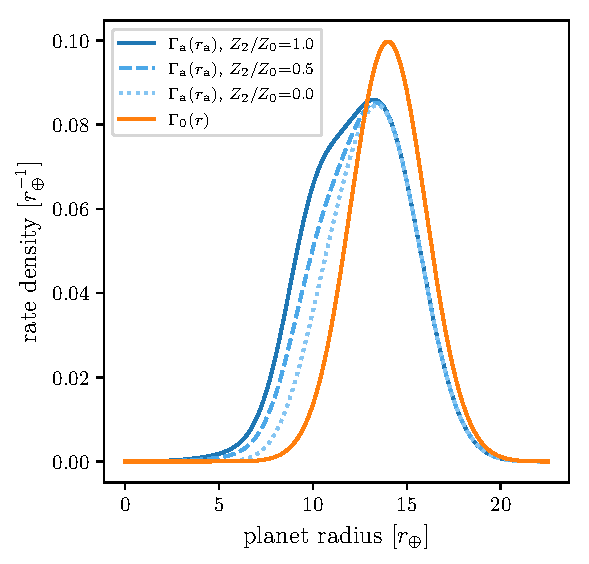
\includegraphics[width=.6\textwidth]{figures/int_rate_density_vs_radius_model_7_rpu_22.5_manyZs.pdf}
    \caption{
        Rate density for a population of planets with true radii $r$
        drawn from a Gaussian with mean $14r_\oplus$ and standard
        deviation $2r_\oplus$.  This is similar to the hot Jupiter
        distribution presented by~\citet{petigura_CKS_2017}.
    }
    \label{fig:gaussian_HJ}
\end{figure}


%%%%%%%%%%%%%%%%%%%%%%%%%%%%%%%%%%%%%%%%%%%%%%%%%%%%%%%%%%%%%%%%%%%%%%%%%%%%%%%
%%%%%%%%%%%%%%%%%%%%%%%%%%%%%%%%%%%%%%%%%%%%%%%%%%%%%%%%%%%%%%%%%%%%%%%%%%%%%%%

\section{Discussion}
\label{sec:discussion}


\paragraph{How bad is ignoring binarity?}
This study has shown that under a reasonable set of simplifying
assumptions, ignoring binarity introduces systematic errors to star
and planet counts in transit surveys, which then biases derived
occurrence rates.  Thus far, occurrence rate calculations\footnote{ A
list of occurrence rate papers is maintained at
\url{https://exoplanetarchive.ipac.caltech.edu/docs/occurrence_rate_papers.html}
} using transit survey data have mostly ignored stellar
multiplicity~\citep[\textit{e.g.},][]{howard_planet_2012,fressin_false_2013,foreman-mackey_exoplanet_2014,dressing_occurrence_2015,burke_terrestrial_2015}.
For {\it Kepler} occurrence rates specifically, it seems that no one
has yet carefully assessed binarity's importance, or lack thereof.
Although this study does not resolve the problem, it does suggest the
approximate scale of the possible errors in a survey-independent
manner.  The suggestion of Section~\ref{sec:model_2} is that for $r\a
\gtrsim 2r_\oplus$, binarity can be ignored down to a precision of a
few percent.  For apparent radii $\lesssim 2r_\oplus$, the picture is
less forgiving: Section~\ref{sec:model_3} suggests that relative
differences between apparent rates and true rates around singles could
easily reach $\sim\! 50\%$.

\paragraph{The rate of Earth analogs}
In line with {\it Kepler}'s primary science goal, the rate of
Earth-like planets orbiting Sun-like stars has been independently
measured by
\citet{youdin_exoplanet_2011,petigura_prevalence_2013,dong_fast_2013,
foreman-mackey_exoplanet_2014}, and \citet{burke_terrestrial_2015}.
These efforts found that the one-year terrestrial planet occurrence
rate is between $\approx\! 0.03$ and $\approx\!1$ per Sun-like star,
depending on assumptions that are made when calculating the
rate~\citep[see][Figure~17]{burke_terrestrial_2015}.  In
Section~\ref{sec:model_3}, our power law model indicates that when
primaries, singles, and secondaries host the same number of planets,
the apparent rate is 50\% higher than the true rate around single
stars.  Though this bias seems large, it is currently smaller than the
other systematic factors that dominate the dispersion in $\eta_\oplus$
measurements.  If future analyses determine absolute values of
$\eta_\oplus$ to better than a factor of two, binarity will likely
merit closer attention.

One caveat to our assessment of binarity's relevance for $\eta_\oplus$
measurements is that none of our models included the rate density's
period-dependence. However, binaries with separations $\lesssim
10\,{\rm AU}$ could provoke dynamical instabilities, leading to fewer
Earth-like planets per
star~\citep[\textit{e.g.},][]{holman_long-term_1999,wang_influence_2014,
kraus_impact_2016}.  This would affect transit survey measurements of
$\eta_\oplus$ beyond our rough estimate.

\paragraph{Hot Jupiter rate discrepancy}
While binarity may appreciably affect $\eta_\oplus$ measurements, our
analysis suggests that it is unlikely to influence the hot Jupiter
rate discrepancy.  The context of this disagreement is that hot
Jupiter occurrence rates measured by transit surveys ($\approx 0.5\%$)
are marginally lower than those found by radial velocity surveys
($\approx 1\%$; see Table~\ref{tab:hj_rates}).  Though the discrepancy
has weak statistical significance ($<3\sigma$), one reason to expect a
difference is that the corresponding stellar populations have distinct
metallicities.  As argued by \citet{gould_frequency_2006}, the RV
sample is biased towards metal-rich stars, which have been measured by
RV surveys to preferentially host more giant
planets~\citep{santos_spectroscopic_2004,fischer_planet-metallicity_2005}.
Investigating the discrepancy from the metallicty
angle,~\citet{guo_metallicity_2017} measured the {\it Kepler} field's
mean metallicity to be $[{\rm M/H}]_{\rm Kepler}= -0.045\pm0.009$,
which is lower than the California Planet Search's mean of $[{\rm
M/H}]_{\rm CPS}= -0.005\pm0.006$.  The former value agrees with that
measured by \citet{dong_metallicities_2014}.  Refitting for the
metallicity exponent in $\Lambda_{\rm HJ} \propto 10^{\beta [{\rm
M/H}] }$, \citeauthor{guo_metallicity_2017}\! found $\beta = 2.1\pm
0.7$, and noted that this would imply that the metallicity difference
could account for a $\approx 20\%$ relative difference in the measured
rates between the CKS and {\it Kepler}\ samples~--~not a 50\% relative
difference\footnote{ \citet{petigura_CKS_2017} recently found $\beta =
3.4^{0.9}_{-0.8}$.  This gives a $\approx 25\%$ relative difference,
indicating metallicity could account for about half of the ``hot
Jupiter rate discrepancy''.  }.  \citeauthor{guo_metallicity_2017}\!
concluded that ``other factors, such as binary contamination and
imperfect stellar properties'' must also be at play.

Binarity might affect the inferred occurrence rates because 
radial velocity and transit surveys treat binaries differently.
Radial velocity surveys typically reject both visual and spectroscopic
binaries \citep{wright_frequency_2012}.  Transit
surveys observe binaries, but the question of whether they were
searchable to begin with is left for later interpretation.  In
spectroscopic follow-up of transiting planet candidates, the
prevalence of astrophysical false-positives may also lead to a
tendency against confirming transiting planets in binary systems.  A
separate observational bias is that the RV surveys typically observe
chromospherically ``quiet'' stars, which may bias their detection
probability high~\citep{bastien_radial_2014}.

Ignoring these complications, we concentrated in this work on
binarity's effects on star counts and the apparent radii of detected
planets.  Assuming a power law radius distribution, and that no
secondaries host HJs, we found in Section~\ref{sec:model_3} that
binarity could lead to underestimated HJ rates relative to singles by
a multiplicative factor of $\approx 1.13$.  We then pointed out in
Section~\ref{sec:further_models} that assuming a power law radius
distribution is probably wrong if one wishes to study the HJ rate
discrepancy.  If we instead assume a Gaussian radius
distribution~\citep[following][]{petigura_CKS_2017}, apparent HJ rates
are {\it greater} than the true rate around singles: the effect goes
the wrong way.
\begin{comment}
  If we believe the assumed power law radius distribution, we can ask
  whether this ``correction factor'' might help resolve the
  discrepancy.  Explicitly, we ask: what is the probability of
  \citet{wright_frequency_2012}'s result, given a rate drawn from the
  stated bounds of~\citet{petigura_CKS_2017}?  In other words, we
  first take the true HJ rate per thousand stars as $\Lambda_{\rm HJ}
  = 5.7 \pm 1.3$, with Gaussian uncertainties.  We then draw from a
  Poisson distribution and compute the probability of detecting at
  least 10 hot Jupiters in a sample of 836 stars.  Without accounting
  for binarity or metallicity, only 4\% of RV surveys would detect at
  least 10 hot Jupiters.  If we multiply $\Lambda_{\rm HJ}$ by $1.2$
  to account for~\citet{guo_metallicity_2017}'s measured metallicity
  difference between the {\it Kepler}\ field and the local solar
  neighborhood, 9\% of RV surveys would detect at least 10 hot
  Jupiters.  If we multiply once more by $1.13$ to account for
  binarity's supposed bias, we find that 14\% of RV surveys would
  detect at least 10 hot Jupiters, still suggesting a weak
  discrepancy.  This suggestion should be taken with caution, because
  it (incorrectly) assumes a power law radius distribution.
\end{comment}
The ``hot Jupiter island'' reported by~\citet{petigura_CKS_2017}
cannot possibly be part of a continuous power law.  Thus binarity is
unlikely to resolve the HJ rate discrepancy.

\begin{comment}
  Of course, such calculations are only suggestive; a conclusive
  resolution of binarity's effects may require a detailed
  understanding of the {\it Kepler}\ field's multiplicity statistics,
  and the mission's completeness (both for candidate detection and
  follow-up).  For instance, if hot Jupiters are less likely to be
  confirmed in binary systems, this might bias the rates low.
  Alternatively, {\it TESS}\ is expected to discover over $10^4$ giant
  planets~\citep{ricker_transiting_2014,sullivan_transiting_2015}.
  Though they will be difficult to distinguish from false positives,
  one possible use of this sample will be to measure an occurrence
  rate of short-period giant planets with minimal error from counting
  statistics.  Our models suggest that binarity will only become an
  appreciable fraction of the error budget at the $\approx 10\%$
  precision level.  This should be sufficient for a rate measurement
  precise enough to indicate a preference between $\approx 0.5\%$ and
  $\approx 1\%$ of Sun-like stars hosting hot Jupiters.
\end{comment}


\paragraph{Practical effects: smooth detection efficiencies; finite SNR floors}
To apply this study to real transit surveys, a few practical concerns
become pressing.  One issue is that space-based missions with
telemetric requirements are often required to select target stars.
Even if the selection process aims to create an SNR-limited
survey, as~\citet{batalha_selection_2010} did for {\it Kepler},
uncertainties in stellar parameters and the modeled instrument
performance can lead to deviations away from an SNR-limited stellar
sample.

Another concern is that in most transit surveys the detection
efficiency is not a step function in SNR.  Transit survey pipeline
detection efficiencies are usually smooth functions~--~see for example
the injection-recovery simulations performed
by~\citet{christiansen_measuring_2016} on {\it Kepler}\ data, and the
resulting detection efficiency adopted
by~\citet{fulton_california-_2017}.  If we were to assume a smooth
detection probability in SNR, we would need to include a detection
efficiency term in Equation~\ref{eq:apparent_rate_density} to
inversely weight for planets with low probabilities of being detected.

The simplest way to avoid the conceptual complications of accounting
for finite detection efficiency is to raise the SNR floor, to {\it
e.g.,} ${\rm SNR} \approx 12$ for {\it Kepler}
(\citealt{fulton_california-_2017}, Figure~5).  To a good
approximation, this allows one to use the boolean distinctions
``searchable'' and ``not searchable'' for signals of an observed depth
(at fixed orbital period).  By making the survey strictly SNR-limited,
rather than ``fuzzily SNR-limited'', binarity's effects become much
easier to model.  Since the minimum SNR for detection is set in an
arbitrary manner anyway\footnote{For example, {\it Kepler}'s threshold
of ${\rm SNR}=7.1$ was set for there to be no more than one
statistical false alarm across the full {\it Kepler}
campaign~\citep{jenkins_tests_2002}. Equally valid would have been to
insist on no more than $10^{-3}$ false alarms per survey, raising the
detection floor.  }, this simplification would put occurrence rate
studies on clearer conceptual ground, and facilitate the process of
converting the observed distributions of apparent radii into true
radius distributions.

Finally, our calculations also ignore the fact that any given transit
survey's finite SNR floor might censor the apparent rate density.  If
the surveyed stars all have the same size, this is equivalent to
saying that there might be a cutoff in apparent planet radii, below
which no planets are detected.  The effects on 
Figures~\ref{fig:occ_rate_model_3_log},~\ref{fig:frac_model_3},
and~\ref{fig:gaussian_HJ} would be that the apparent rate density
below the cutoff in apparent radius would simply drop to zero.

\begin{comment}
  If one insists on using a smooth detection efficiency, then life
  probably becomes more complicated.  It might then be necessary to
  model the detection pipeline's efficiency while somehow
  marginalizing over binarity.  Since the relative number of
  detections (at fixed $\delta_{\rm obs}$) coming from singles,
  primaries, and secondaries changes as a function of the intrinsic
  distribution of planet parameters (Figure~\ref{fig:frac_model_3}),
  some complicated deconvolution might be required.
\end{comment}



\paragraph{Connecting high resolution imaging to occurrence rates}
One reason to address stellar multiplicity in transit surveys is that
it can radically alter the interpretation of planet candidates on a
system-by-system level.  Consequently, high resolution imaging
campaigns have measured the multiplicities of almost all {\it Kepler}\
Objects of Interest~\citep{
  howell_speckle_2011,adams_adaptive_2012,adams_adaptive_2013,horch_observations_2012,
  horch_most_2014,lillo-box_multiplicity_2012,lillo-box_high-resolution_2014,dressing_adaptive_2014,
  law_robotic_2014,cartier_revision_2015,everett_high-resolution_2015,gilliland_hubble_2015,
  wang_influence_2015,wang_influence_2015-1,baranec_robo-ao_2016,ziegler_robo-ao_2017}.
The results of these programs have been collected
by~\citet{furlan_kepler_2017}, and they represent an important advance
in understanding the KOI sample's multiplicity statistics.  
An immediate application is to reassess the radii of detected planets.
Doing so, \citet{hirsch_assessing_2017} find that for their sample of KOIs
in binaries, the planet radii are underestimated by factors $r/r\a = 1.17$
if all planets orbit primaries, and $r/r\a = 1.65$ if detected
planets are equally likely to orbit primaries and singles.
%In particular, they can be immediately applied to rectify binarity's
%effects on the mass-radius diagram~\citep{furlan_densities_2017}.

These results are beginning to connect with
occurrence rate calculations: using~\citet{furlan_kepler_2017}'s
catalog, recent studies have tested the effects of removing KOI hosts with
known companions, reducing contamination in the ``numerator'' of the
occurrence rate (\citealt{fulton_california-_2017};
\citealt{petigura_CKS_2017}).  
While these are good first steps, the
denominator remains uncorrected.  To count the number of stars that
were searched, further effort to understand the multiplicity
statistics of KOI vs.~non-KOI stars is necessary. In particular,
a non-KOI star high-resolution imaging effort could help estimate
the systematic errors incurred by assuming all surveyed stars are
single.
An alternate approach would be to combine {\it Gaia}
parallaxes with measured photometric fluxes and identify binary systems
as those that are 
overluminous~\citep[\textit{e.g.},][]{widmark_inferring_2018}.

\paragraph{Does a detected planet orbit the primary or secondary?}
An important step towards rectifying binarity's effects is
identifying the transit host star for detected planets in binaries.
The current wisdom is that, unless the planet can be confirmed to
orbit either component through analysis of the transit durations or
centroids, little can be said about the likelihood of a
planet orbiting the primary vs.~the
secondary~\citep[\textit{e.g.},][though~\citealt{hirsch_assessing_2017}'s 
do weight radius corrections by planet 
occurrence]{ciardi_understanding_2015,ziegler_robo-ao_2017}.

\begin{comment}
  \citet{ciardi_understanding_2015} studied the effects of stellar
  multiplicity on the planet radii derived from transit surveys.  They
  modeled the problem for {\it Kepler}\ objects of interest by
  matching a population of binary and tertiary companions to KOI
  stars, under the assumption that the KIC-listed stars were the
  primaries.  They then computed planet radius correction factors
  assuming that {\it Kepler}-detected planets orbited the primary or
  companion stars with equal probability (their Section~5).  Under
  these assumptions, they found that any given planet's radius is on
  average underestimated by a multiplicative factor of $\approx\!
  1.5$.  \citet{ziegler_robo-ao_2017} recently reported a similar mean
  radius correction factor for the multiple systems observed by the
  Robo-AO KOI survey, using the same assumption that detected planets
  are as likely to orbit the primary and the secondary.
\end{comment}

Assuming a broken power law radius distribution, we showed in
Figure~\ref{fig:frac_model_3} that detected planets in binary systems
are usually more likely to orbit the primary.  A planet orbiting the
secondary does lead to extreme corrections.  However, at $r\a \gtrsim
2r_\oplus$, these cases are rare outliers.  At $r_\oplus \lesssim r\a
\lesssim 2r_\oplus$, for all of the trial values of $Z_2/Z_0$ assumed
in Figure~\ref{fig:frac_model_3}, a detected planet is always more
likely to orbit the primary than the secondary.  Only at very small
apparent radii, $r\a \approx 0.5r_\oplus$, and only if secondaries
host as many planets as singles and primaries, does this ``rule''
break down.

Of course, our model's assumptions (see the list in
Section~\ref{sec:conclusion}) might not apply to the {\it Kepler}\
dataset.  However if they are applicable, then for the $56\%$ of
``\texttt{CONFIRMED}'' KOIs\footnote{Exoplanet Archive;
\cite{akeson_nasa_2013}; \url{exoplanetarchive.ipac.caltech.edu}} with
apparent radii $>2r_\oplus$, whenever high-resolution imaging
discovers a binary companion in a system that hosts a detected
transiting planet, the planet is much more likely to orbit the
primary.


\paragraph{Fraction of detected planets with binary companions vs. apparent 
radius}
One further prediction of Figure~\ref{fig:frac_model_3} is that the
fraction of detected planets with binary companions increases by
$\approx 6-12\%$ going from $2r_\oplus$ to $\approx\! 1.4r_\oplus$.
In \citet{ziegler_robo-ao_2017}'s recent summary of the Robo-AO KOI
survey, they reported the fraction of planet-hosting stars with
Robo-AO detected companion stars, binning by Earths ($r\a <
1.6r_\oplus$), Neptunes ($1.6r_\oplus < r\a < 3.9 r_\oplus$), Saturns
($3.9r_\oplus < r\a < 9 r_\oplus$), and Jupiters ($r\a > 9r_\oplus$).
The reported nearby star rates and their $1\sigma$ uncertainties are:
\begin{itemize}
    \item Earths: $16.3 \pm 1.0\%$, from 1480 systems.
    \item Neptunes: $13.0 \pm 0.8\%$, from 2058 systems.
    \item Saturns: $13.6 \pm 2.0\%$, from 338 systems.
    \item Jupiters: $19.0 \pm 2.8\%$, from 247 systems.
\end{itemize} 
where the uncertainties were calculated
following~\citet{burgasser_binarity_2003}.  The absolute values of the
rates are less than the $\sim\! 45\%$ typical for Sun-like stars at
least in part because of Robo-AO's sensitivity
(\citealt{ziegler_robo-ao_2017}'s
Figure~2;~\citealt{raghavan_survey_2010}).  Another reason for the
lower measured companion rates could be that planetary systems are
less likely to have binary companions (as~\citealt{kraus_impact_2016}
argued for close binary companions).  The uptick in the companion rate
for Jupiters is likely tied to a large astrophysical false positive
rate~\citep{santerne_sophie_2012}.  Going from Neptunes to Earths, the
data suggest a weak increase in the detected planet companion
fraction, perhaps of a few percent.  It will be interesting to see
whether this effect is borne out by further observations.


\begin{comment}
  \paragraph{Independent approaches for estimating binarity's effects}
  T. Barclay et al.\! (in preparation) have performed the exercise of
  taking stars selected by the {\it Kepler}\ team, pairing them with a
  population of secondaries, injecting a realistic distribution of
  planet radii, and then comparing the inferred occurrence rates with
  the true ones.  In their model, they find that binarity leads to an
  inferred rate of Earth-sized planets $\approx 10\%$ less than the
  true rate.  In our Model \#3, if all $Z_i$'s are equal (a plausible
  assumption in the lack of evidence to the contrary), the
  underestimate is by a comparable 16\%.
\end{comment}

%%%%%%%%%%%%%%%%%%%%%%%%%%%%%%%%%%%%%%%%%%%%%%%%%%%%%%%%%%%%%%%%%%%%%%%%%%%%%%%
%%%%%%%%%%%%%%%%%%%%%%%%%%%%%%%%%%%%%%%%%%%%%%%%%%%%%%%%%%%%%%%%%%%%%%%%%%%%%%%

\section{Conclusion}
\label{sec:conclusion}

This study presented simple models for how binarity affects occurrence
rates measured by transit surveys.  The simplest of these models
(Section~\ref{sec:simplest}) provided an order-of-magnitude estimate
that suggested we would need implausibly high twin binary fractions
for binarity to affect apparent occurrence rates by more than factors
of two.

We then derived a general formula for the apparent rate density
inferred by an observer ignoring binarity
(Equation~\ref{eq:general_Gamma_a}).  As input, this equation requires
a volume-limited mass ratio distribution $f(q)$, and the true rate
densities for planets around singles, primaries, and secondaries.  The
assumptions that make the model tractable are:
\begin{enumerate}
    \item the transit survey is SNR-limited;
    \item the true properties of all the singles and primaries are
      known to the observer;
    \item the observers assume that binaries have the same properties
      as the primaries;
    \item there are functions $L(M)$ and $R(M)$ that specify a star's
      luminosity and radius in terms of its mass.
\end{enumerate}
Allowing for these conditions, many results follow:
\begin{itemize}
%
\item Assuming a power law planet radius distribution, and that the
  same number of planets orbit singles, primaries, and secondaries,
    binarity influences apparent planet occurrence rates around
    Sun-like stars at the $\sim$few percent level from radii
    $2r_\oplus \lesssim r\a \lesssim 17r_\oplus$
    (Section~\ref{sec:model_2}).
%
\item Assuming a broken-power law planet radius distribution, with
  \citet{howard_planet_2012}'s exponent at $r > 2r_\oplus$ and a
    constant occurrence at $r < 2r_\oplus$, there is a ``bump'' in the
    apparent rate density at $r\a < 2r_\oplus$, leading to a relative
    error $\delta \Gamma_0 = |\Gamma_0 - \Gamma\a|/\Gamma_0$ of at
    most $\approx 50\%$ (Figure~\ref{fig:occ_rate_model_3_log}).
    Although this is smaller than current systematic uncertainties on
    the occurrence rates of Earth-sized planets, this means that
    binarity could eventually become an important component of the
    $\eta_\oplus$ error budget.
%
\item Binarity ``fills in'' gaps in the radius distribution
  (Figure~\ref{fig:model_4}), by an amount that could affect precise
    measurements of the depth, width, and slope of
    \citet{fulton_california-_2017}'s radius gap, in the event that
    planets are not carefully vetted with high resolution imaging.
%
\item Binarity does not lead to smaller apparent HJ occurrence rates
  (Figure~\ref{fig:gaussian_HJ}).  This assumes a Gaussian planet
    radius distribution, similar to that reported
    by~\citet{petigura_CKS_2017}.
%
\item Detected planets with $r\a \gtrsim 0.5r_\oplus$ that are
  revealed by high resolution imaging surveys to exist in binaries are
    more likely to orbit the primary (Figure~\ref{fig:frac_model_3}).
%
\item Near the ``break'' in the rate distribution ($\approx
  2r_\oplus$), the fraction of detected planets with binary companions
    increases by $\approx 5-10\%$ (Figure~\ref{fig:frac_model_3}).
\end{itemize}

All of these results should be understood as only being strictly
applicable when the assumptions listed above are met.  Otherwise,
while it is only suggestive, our approach still provides helpful hints
at how ignoring stellar binarity influences transit survey occurrence
rates.



\acknowledgements{
It was a pleasure discussing this study with T.~Barclay, W.~Bhatti,
J.~Christiansen and F.~Dai.  This work made use of NASA's Astrophysics
Data System Bibliographic Services.
%
\newline
%
\software{\texttt{numpy}~\citep{walt_numpy_2011}, 
\texttt{scipy}~\citep{jones_scipy_2001}, 
\texttt{matplotlib}~\citep{hunter_matplotlib_2007}, 
\texttt{pandas}~\citep{mckinney-proc-scipy-2010}
}
}

\newpage
\appendix
\section{Derivation of general formula for apparent occurrence rate}
\label{sec:appendix}

This appendix derives Equation~\ref{eq:general_Gamma_a} in a more
rigorous manner than in Section~\ref{sec:general_formula}.  First,
recall our definition of apparent rate density
(Equation~\ref{eq:apparent_rate_density}).  We assume that $R$ and $L$
are uniquely determined from the assumed stellar
mass--radius--luminosity relation, and neglect the dependence on
planetary orbital period.  The planets with $(r\a, M\a)$ are
associated with systems of many different planetary and stellar
properties, so $n_{\rm det}(r\a, M\a)$ is given by the convolution of
the true rate density, $\Gamma(r, M)$, and $\mathcal{N}_\star(r\a,
M\a; r, M)$, the number (per unit $(r\a, M\a)$) of searchable stars
that give $(r\a, M\a)$  when the true system actually has $(r, M)$.
Mathematically,
\begin{align}
    n_{\rm det}(r\a, M\a) &=
    \sum_i n_{\rm det}^i(r\a, M\a) \\
    &=
    \sum_i \int \mathrm{d}r \mathrm{d}M \,
    \mathcal{N}_\star^i(r\a,M\a; r,M)
    \cdot\Gamma_i(r,M) \cdot p_{\rm tra}(r,M),
    \label{eq:n_det}
\end{align}
where $i$ specifies the type of true host stars (0: single, 1:
primary, 2: secondary).  The problem reduces to the evaluation of
\begin{equation}
    \mathcal{N}_\star^i(\pp\a,\ps\a; \pp, \ps)
\end{equation}
for planets around single stars, primaries in binaries, and
secondaries in binaries. 

\paragraph{Single stars} For $i=0$, 
\begin{equation}
    \mathcal{N}_\star^0(r\a,M\a; r,M)
    =\delta(r\a-r)\delta(M\a-M) N_\star^0(r,M),
\end{equation}
so
\begin{equation}
    n_{\rm det}^0(r\a, M\a)=N_\star^0(r\a,M\a)\cdot \Gamma_0(r\a, 
    M\a) \cdot p_{\rm tra}(r\a, M\a).
\end{equation}

\paragraph{Primaries in binaries}
The number of primaries with apparent parameters $(r\a,M\a)$ given the
true parameters $(r,M)$ is
\begin{equation}
    \mathcal{N}_\star^1(r\a, M\a; r, M)
    = \int 
      \mathrm{d}q\,f(q)\mathcal{N}_{{\rm s}, q}^1(r\a, M\a, q; r, M),
    \label{eq:fancyN_s_1}
\end{equation}
where $f(q)$ is the volume-limited binary mass ratio distribution.

Since we assume $\ps\a=\ps_1$,
\begin{equation}
    \mathcal{N}_{{\rm s},q}^1(r\a, M\a, q; r, M)
    \propto
    \delta(M\a-M).
\end{equation}
In this case, $\mathcal{N}_{{\rm s},q}^1$ is non-zero only at
$r\a=R\a\sqrt{\delta_{\rm obs}}$, and the observed depth is
\begin{equation}
    \delta_{\rm obs}
    = \left[{r\over R(M\a)}\right]^2\times {L(M\a) \over L_{\rm sys}(M\a, q)}
    \equiv \left[{r\over R(M\a)}\right]^2\times \mathcal{A}(q,M\a)^2,
    \label{eq:delta_obs_primaries} 
\end{equation}
where
\begin{equation}
    \mathcal{A}(q, M\a)=\sqrt{L(M\a) \over L_{\rm sys}(M\a, q)}.
\end{equation}
The normalization of $\mathcal{N}_{{\rm s},q}^1$ is given by the
number of binaries that are searchable for a signal $\delta_{\rm obs}$
and that have the mass ratio $q$:
\begin{equation}
    N_\star^0(\delta_{\rm obs}, 
    L(M\a))\cdot
    {n\b\over n\s}\left[L_{\rm sys}(M\a, q) \over L(M\a)\right]^{3/2}
    =N_\star^0(\delta_{\rm obs}, L(M\a))
    \cdot \frac{{\rm BF}}{1 - {\rm BF}} \cdot {1 \over \mathcal{A}(q,M\a)^3}.
    \label{eq:primary_normalization}
\end{equation}
Thus,
\begin{align}
    \notag
    \mathcal{N}_{{\rm s}, q}^1(r\a, M\a, q; r, M)
    &=N_\star^0(\delta_{\rm obs}, L(M\a))
    \cdot \frac{{\rm BF}}{1 - {\rm BF}} \cdot {1 \over \mathcal{A}(q,M\a)^3}\\
    &\times\delta \left[r\a-r\mathcal{A}(q,M\a)\right]\delta(M\a-M).
    \label{eq:N_s_1}
\end{align}


\paragraph{Secondaries in binaries}
In this case, $M=qM_1=qM\a$, so
\begin{equation}
    \mathcal{N}_{{\rm s},q}^2(r\a, M\a, q; r, M)
    \propto \delta\left(M\a-{M\over q}\right).
    \label{eq:fancyN_s_2_prop}
\end{equation}
Again $\mathcal{N}_\star^2$ is non-zero only at
$r\a=R\a\sqrt{\delta_{\rm obs}}$, but this time
\begin{equation}
    \delta_{\rm obs} = \left[{r\over R(qM\a)}\right]^2 \times {L(qM\a) 
      \over L_{\rm sys}(M\a, q)}
      \equiv \left[{r\over R(M\a)}\right]^2\times \mathcal{B}(q,M\a)^2,
\end{equation}
where
\begin{equation}
    \mathcal{B}(q, M\a)={R(M\a)\over R(qM\a)}\sqrt{{L(qM\a) \over
    L_{\rm sys}(M\a, q)} }.
\end{equation}
The normalization remains the same as the previous case (we are
counting the searchable stars at a given observed depth $\delta_{\rm
obs}$, and the total luminosity of the binary is the same).  Thus,
\begin{equation}
    \mathcal{N}_\star^2(r\a, M\a; r, M)
    =\int \mathrm{d}q\,f(q)\mathcal{N}_{{\rm s}, q}^2(r\a, M\a, q; r, M),
\end{equation}
where
\begin{align}
    \notag
    \mathcal{N}_{{\rm s},q}^2(r\a, M\a, q; r, M)
    &=N_\star^0(\delta_{\rm obs}, L(M\a)) \cdot \frac{{\rm BF}}{1 - {\rm BF}} 
    \cdot {1 \over \mathcal{A}(q,M\a)^3}\\
    &\times 
      \delta \left[r\a-r\mathcal{B}(q,M\a)\right]
      \delta\left(M\a-{M\over q}\right).
    \label{eq:mathcal_N_s_2}
\end{align}

One might worry in Equation~\ref{eq:mathcal_N_s_2} that we opt to
write $\mathcal{N}\s^2 \propto \delta(M\a - M/q)$, rather than
$\propto \delta(M\a q - M)$ or some other delta function with the same
functional dependence, but a different normalization once integrated.
We do this because the delta function in
Equation~\ref{eq:mathcal_N_s_2} is defined with respect to the measure
${\rm d}M\a$, not ${\rm d}M$.  This is because $\mathcal{N}\s^2$ is
defined as a number per $r\a$, per $M\a$.

\paragraph{Number of detected planets}
Marginalizing per Equation~\ref{eq:n_det}, we find
\begin{align}
    \notag
    n_{\rm det}^0(r\a, M\a)
    &=\int\mathrm{d}r\mathrm{d}M\,\mathcal{N}_\star^0(r\a, M\a; r, M)
    \cdot\Gamma_0(r, M) \cdot p_{\rm tra}(M)\\
    &=N_\star^0(\delta_{\rm obs}, L(M\a))\cdot\Gamma_0(r\a, M\a) \cdot p_{\rm 
        tra}(M\a),
    \label{eq:n_det_0}
\end{align}
and
\begin{align}
    \notag
    n_{\rm det}^1(r\a, M\a)
    &=\int\mathrm{d}r\mathrm{d}M\,\mathcal{N}_\star^1(r\a, M\a; r, M)
    \cdot\Gamma_1(r, M) \cdot p_{\rm tra}(M)\\
    &=N_\star^0(\delta_{\rm obs}, L(M\a))\cdot p_{\rm tra}(M\a) \cdot
    {\mathrm{BF}\over{1-\mathrm{BF}}} \int {\mathrm{d}q \over 
        \mathcal{A}^4}\,f(q)\,\Gamma_1\left({r\a\over\mathcal{A}}, M\a\right).
    \label{eq:n_det_1}
\end{align}
Finally,
\begin{align}
    n_{\rm det}^2(r\a, M\a)
    \notag
    &=\int\mathrm{d}r\mathrm{d}M\,\mathcal{N}_\star^2(r\a, M\a; r, M)
    \cdot\Gamma_2(r, M) \cdot p_{\rm tra}(M)\\
    &=
    N_\star^0(\delta_{\rm obs}, L(M\a))\cdot \frac{{\rm BF}}{1 - {\rm BF}}
    \int {q \mathrm{d}q \over 
    {\mathcal{A}^3\mathcal{B}}}\,f(q)\,\Gamma_2\left({r\a\over\mathcal{B}}, 
    qM\a\right)\,p_{\rm 
        tra}(qM\a).
    \label{eq:n_det_2}
\end{align}


\paragraph{General formula for apparent occurrence rate}
Using the above results, the apparent rate density,
\begin{align}
    \Gamma\a(r\a,M\a) &= 
    \frac{1}{N_\star(r\a,M\a) p_{\rm tra}(r\a,M\a)} \times
    \sum_i n_{\rm det}^i (r\a,M\a),
\end{align}
evaluates to

\begin{align}
    \notag
    \Gamma\a(r\a,M\a) &= {1\over 1+\mu(\mathrm{BF}, M\a)}\times
    \left\{ \Gamma_0(r\a, M\a)+ 
    \frac{{\rm BF}}{1 - {\rm BF}}
    \left[ \int {\mathrm{d}q \over \mathcal{A}^4}\,f(q)\,\Gamma_1\left({r\a\over 
        \mathcal{A}}, 
    M\a\right)\,
    \right.   
    \right. \\
    & \quad\quad\quad\quad\quad \left.\left.
    +\int {q \mathrm{d}q \over 
        {\mathcal{A}^3\mathcal{B}}}\,f(q)\,\Gamma_2\left({r\a\over 
        \mathcal{B}}, 
    qM\a\right)\,
    {R(qM\a) \over R(M\a)}
    q^{-1/3} \right]	\right\}.
    \label{eq:final_formula}
\end{align}
This equation is used to derive
Equations~\ref{eq:model5_apparent_rate_density}
and~\ref{eq:powerlaw_vary_binary}, and is numerically integrated to
create Figs.~\ref{fig:occ_rate_model_3_log},~\ref{fig:model_4},
and~\ref{fig:gaussian_HJ}.  It is validated in limits in which it is
possible to write down the answer (e.g.,
Equation~\ref{eq:model_1_apparent_rate_density}), and also against a
Monte Carlo realization of the twin binary models
(Secs.~\ref{sec:model_1} and~\ref{sec:model_2}).





\newpage
%% \begin{deluxetable}{} command tell LaTeX how many columns
%% there are and how to align them.
\begin{deluxetable}{cccc}
    
%% Keep a portrait orientation

%% Over-ride the default font size
%% Use Default (12pt)

%% Use \tablewidth{?pt} to over-ride the default table width.
%% If you are unhappy with the default look at the end of the
%% *.log file to see what the default was set at before adjusting
%% this value.

%% This is the title of the table.
\caption{Occurrence rates of hot Jupiters (HJs) about FGK dwarfs, as measured 
by radial velocity and transit surveys.}
\label{tab:hj_rates}

%% This command over-rides LaTeX's natural table count
%% and replaces it with this number.  LaTeX will increment 
%% all other tables after this table based on this number
\tablenum{1}

%% The \tablehead gives provides the column headers.  It
%% is currently set up so that the column labels are on the
%% top line and the units surrounded by ()s are in the 
%% bottom line.  You may add more header information by writing
%% another line between these lines. For each column that requries
%% extra information be sure to include a \colhead{text} command
%% and remember to end any extra lines with \\ and include the 
%% correct number of &s.
\tablehead{\colhead{Reference} & \colhead{HJs per thousand stars} & 
\colhead{HJ Definition} 
%& 
%\colhead{} \\ 
%    \colhead{} & \colhead{(planets per thousand stars)} & \colhead{} & 
%    \colhead{}
} 

%% All data must appear between the \startdata and \enddata commands
\startdata
Marcy+ 2005 & 12$\pm$1 & $a<0.1\,{\rm AU}; P\lesssim10\,{\rm day}$ \\
Cumming+ 2008 & 15$\pm$6 & -- \\
Mayor+ 2011 & 8.9$\pm$3.6 & -- \\
Wright+ 2012 & 12.0$\pm$3.8 & -- \\
Gould+ 2006 & $3.1^{+4.3}_{-1.8}$ & $P<5\,{\rm day}$ \\
Bayliss+ 2011 & $10^{+27}_{-8}$ & $P<10\,{\rm day}$ \\
Howard+ 2012 & 4$\pm$1 & $P<10\,{\rm day}; r_p=8-32r_\oplus$; solar 
subset\tablenotemark{a} \\
-- & 5$\pm$1 & solar subset extended to $Kp<16$ \\
-- & 7.6$\pm$1.3 & solar subset extended to $r_p>5.6r_\oplus$. \\
Moutou+ 2013 & 10$\pm$3 & {\it CoRoT} average; $P\lesssim 10\,{\rm day}$, 
$r_p>4r_\oplus$  \\
Petigura+ (in prep) & 5.7$\pm$1.3 &
    $r_p=8-24r_\oplus$; $1<P/{\rm day}<10$; CKS stars\tablenotemark{b} \\
Santerne+ (in prep) & 9.5$\pm$2.6 & {\it CoRoT} galactic center \\
-- & 11.2$\pm$3.1 & {\it CoRoT} anti-center \\
\enddata

%% Include any \tablenotetext{key}{text}, \tablerefs{ref list},
%% or \tablecomments{text} between the \enddata and 
%% \end{deluxetable} commands

%% General table comment marker
\tablecomments{
    The upper four results are from radial velocity surveys; the rest
    are from transit surveys. Many of these surveys selected different 
    stellar samples. ``--'' denotes ``same as above''.
}
\tablenotetext{a}{
    Howard+ 2012's ``solar subset'' was defined as {\it Kepler}-observed stars 
    with $4100\,{\rm K}<T_{\rm eff}<6100\,{\rm K}$, $Kp <15$, $4.0 < \log g < 
    4.9$. Their rate selected planets with measured signal to noise $>10$.
    }
\tablenotetext{b}{
    Petigura+ (in prep)'s CKS subset included $\ldots$
}   
\end{deluxetable}



\newpage
\bibliographystyle{yahapj}                            
\bibliography{bibliography} 

\end{document}
